\chapter{Our traffic scheduler}
\label{chap02}
%motivation: little config (knobless), fast O(1), QoS aware, scheduler in presence of differentiated services. Would run at simple devices

\begin{figure}
	\centering
	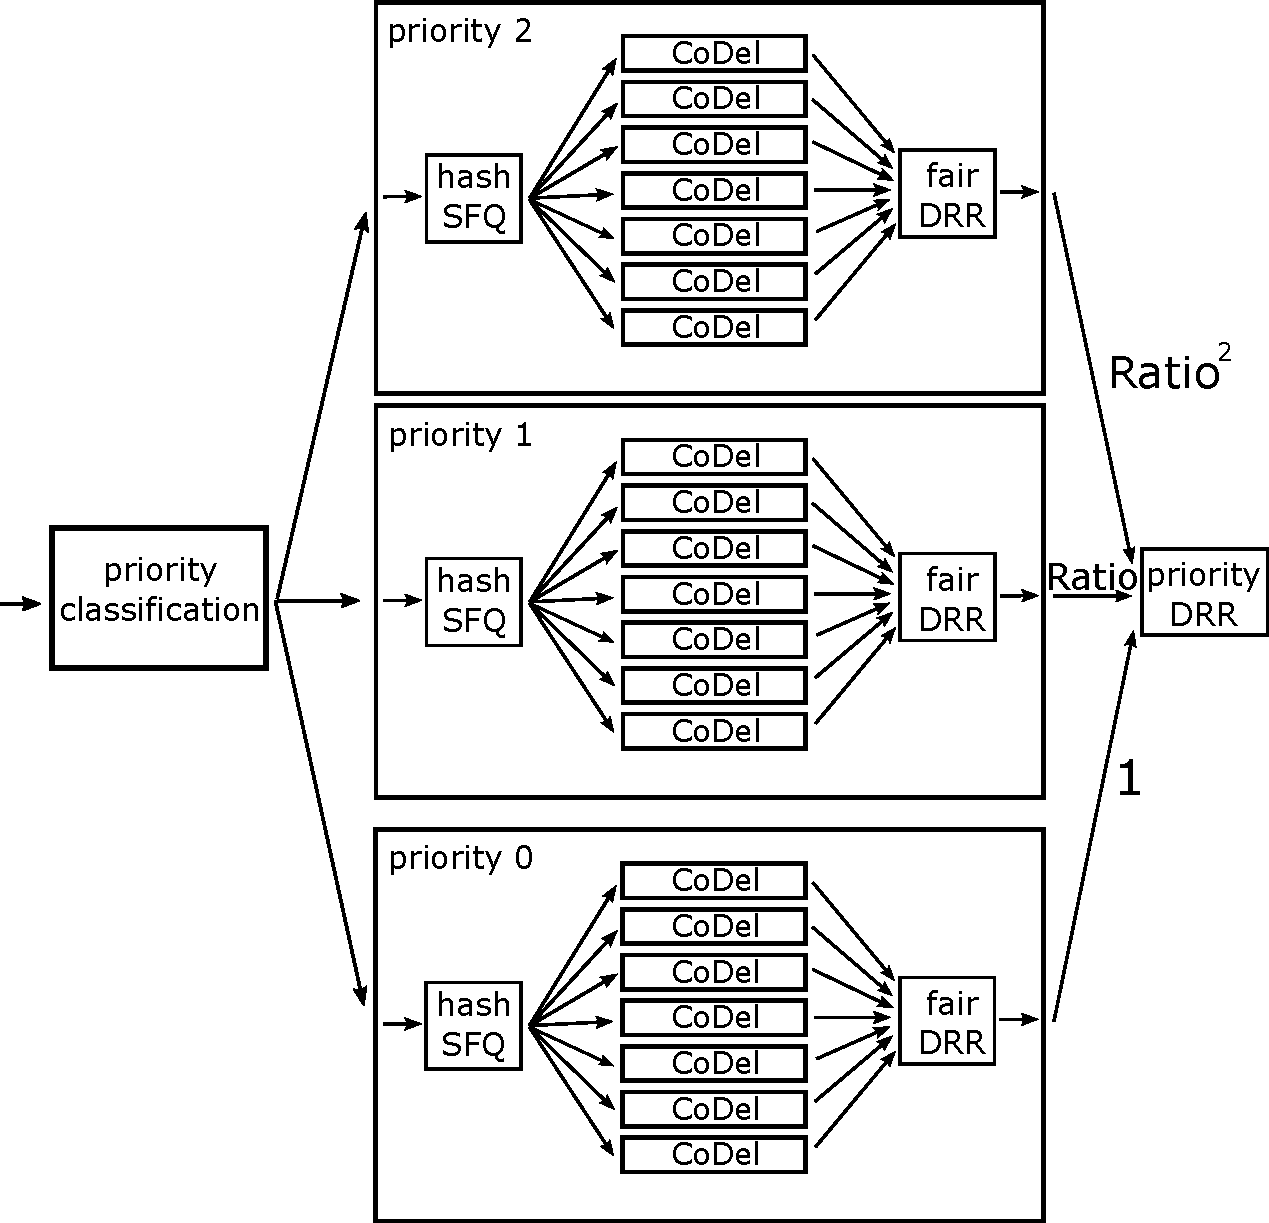
\includegraphics[width=137mm]{drawings/msfc}
	\caption{The MSFC layout}
	\label{fig10:msfc}
\end{figure}

In this thesis, we propose a traffic scheduler Multilevel stochastic fairness queueing (MSFC) illustrated in \ref{fig10:msfc}. It combines ideas of previous work: CoDel and deficit round-robin, to create classful traffic scheduler. It uses three-level layout. In the highest level, packets are assigned to priority classes. We use non-fair DRR to prioritize more important traffic. Inside the classes, packets are distributed into flows (based on source and destination IP addresses, ports and protocol) and we use second, independent fair DRR to schedule traffic within the class. Each flow uses CoDel algorithm.

Additionally, it has following parameters:
\begin{itemize}
	\item $Limit$ --- the maximum amount of packets stored in the qdisc.
	\item $Prios$ --- the number of priority classes (max 8).
	\item $Flows$ --- the number of queues (CoDels) in each priority class (so there is $Prios*Flows$ total independent CoDels)
	\item $Backlog$ --- the maximum backlogged bytes in an individual CoDel.
	\item $Perturb$ --- number of seconds after flow-classification hash function perturbs
	\item $Quantum$ --- the quantum parameter of the inner fair DRR (see \ref{DRR})
	\item $Target$ --- target delay parameter for CoDel algorithm (see \ref{CoDel})
	\item $Interval$ --- Interval parameter for CoDel algorithm (see \ref{CoDel})
	\item $Ratio$ --- defines the ratio of bandwidth of two adjacent priority classes. The ratio is enforced by the outer DRR. MSFC uses $Ratio$ to compute quantums of all priority classes. The quantums rise exponentially:
	\[
	Q_p = Quantum \cdot Ratio^p,
	\]
	where $p$ is the priority of class, and $Quantum$ is the parameter for inner DRR.
\end{itemize}
So if there are 3 classes with priorities 0--2 (like in the Figure \ref{fig10:msfc}), the upstream bandwidth will be distributed in ratio $1:Ratio:Ratio^2$.

Note, that the ratio is independent of the number of flows in each class. Consider two classes with adjacent priorities 0 and 1. Priority 1 class has only one flow backlogged, priority 0 class has 100 flows. The one flow from priority 1 class is guaranteed to receive 2/3 of the bandwidth. The 1/3 is distributed fairly between the remaining 100 flows.

%fq codel -new old distinction vs remembering quantum when deactivating

\section {Implementation}

We have implemented the MSFC algorithm into the Network simulator 3 (ns3) to evaluate in simulated conditions. We have also implementation in Linux kernel for actual deployment in real devices.

\subsection {Linux}
\begin{figure}
	\centering
	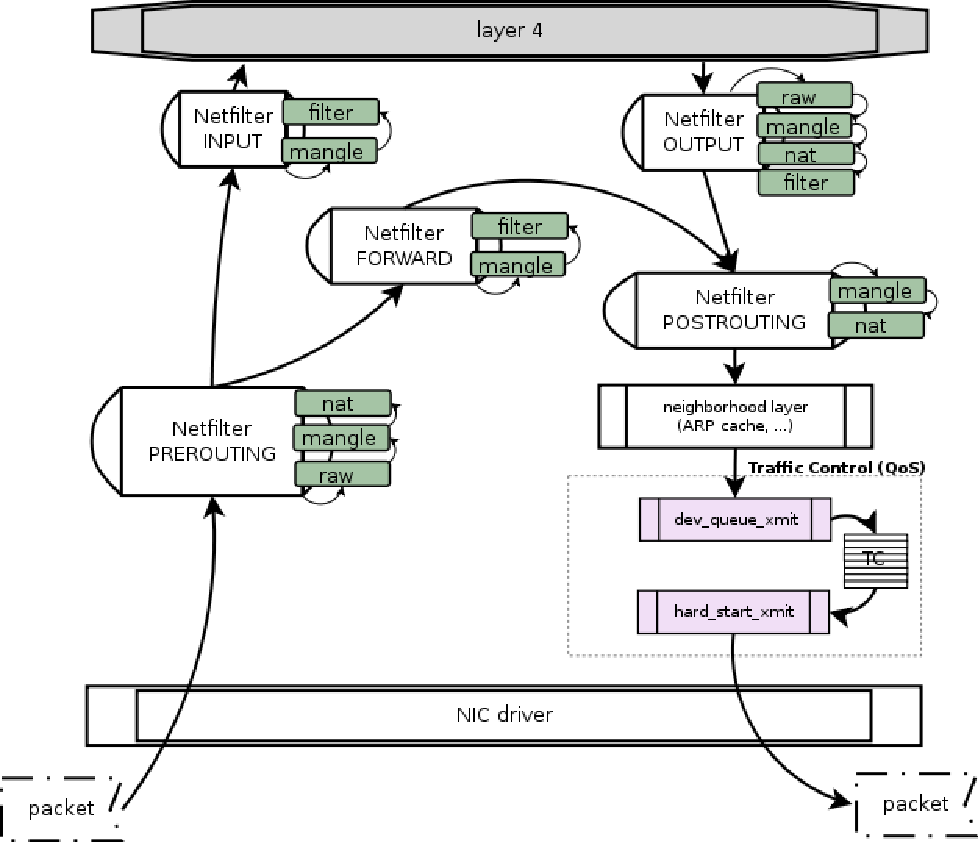
\includegraphics[width=137mm]{drawings/network_stack}
	\caption{Packets traversal through Linux kernel.}
	\label{fig12:linux}
\end{figure}

We have implemented the algorithm into the Linux kernel. To understand the implementation, let us take a look how Linux controls network traffic. The Figure \ref{fig12:linux} shows the context of traffic control in the Linux kernel. It takes place at the bottom of the third (IP) layer, and stores packets that are ready to be handed over to the transport layer.

There are three kinds of objects used in traffic control: qdisc (queuing discipline), class and filter. Simply put, qdisc is traffic scheduler --- its role is to enqueue packets, store them, and choose an outgoing packet when NIC driver asks for one. Every interface must have at least one qdisc --- root qdisc. It may further contain child classes and each class contains exactly one qdisc. Classless qdiscs comprise only one qdisc object. Filter objects allow packet classifying and policing.

When kernel decides a packet is ready to be sent, it enqueues the packet in root qdisc (that exists in every configuration). If the root qdisc is classful, it may end up in any of its child classes. An arbitrary number of filters may be assigned to every class. When a packet arrives to qdisc with multiple child classes, it calls all the filters one by one, until one of them returns with a verdict. The qdisc then enqueues the packet in child qdisc of the chosen class.

However, the concept of classes and filters is not obligatory to use, it depends on implementation of particular queueing discipline. For example, a classful qdisc may not use filters to classify packet, but use a different method instead (e.g. Type of Service field in IP header). Also qdisc may be classless in relation to Linux kernel, but still use internal 'classes' --- treat different groups of packets differently.

In the kernel, packets are represented by struct sk\_buff (socket buffer). This avoids copying of packets and provides us with attributes like pointer to socket where packet was created, timestamps, length, etc. One of the attributes is (queuing) priority. By default, the kernel sets the priority to value of field Type of Service from packet IP header. However, user may configure the system to change the priority in postrouting mangle phase (see Figure \ref{fig12:linux} and thus classify packets even before they come to qdisc.

The default qdisc is pfifo\_fast. It is three-band first-come first-serve scheduler. There are 3 independent FIFO queues, one for each priority. Pfifo\_fast classifies packets based on priority attribute of sk\_buff (it takes 4 least significant bits). The dequeue is simple: it iterates dequeues packet from highest priority non-empty FIFO queue.

Every qdisc is connected to the kernel via struct Qdisc\_ops. It defines pointers to methods that the kernel calls to operate the qdisc. Every qdisc then defines variable of type Qdisc\_ops and assigns implementations of corresponding methods to the members of the struct. The most important members are:



\begin{itemize}
	\item enqueue
	\item dequeue
	\item 
\end{itemize}

We have implemented the MSFC as classless qdisc. There is 

qdisc interface

\subsection {Network simulator 3}

-ns3 --- seeds and replication of results


